\chapter{POTENTIAL DEVELOPMENT SOFTWARE}
\label{ch:software}
\lstset{
	language=python,
	% basicstyle=\small\sffamily,
	numbers=left,
	numberstyle=\tiny,
	% frame=tb,
	columns=fullflexible,
	showstringspaces=false
}
\section{Introduction}

The simulation of atoms involving hundreds of atoms are commonplace, due to the success of density functional theory\cite{hohenberg1964_dft,kohn1965_dft} and the availability of many software packages avail for the calculations such as VASP\cite{kresse1993_vasp,kresse1996_vasp1,kresse1996_vasp2}, ABINIT\cite{gonze2002_abinit,gonze2005_abinit,gonze2009_abinit,gonze2016_abinit}, and Quantum Espresso\cite{giannozzi2009_quantumespresso}.
These electronic-structure calculations are high-fidelity calculations, which accuracy improving as the description of the exchange correlation energy functional has improved from local density approximation(LDA) to PBE to hybrid methods.
These electronic-structure models allow for simulations of hundreds of atoms which when combined with workflow management software, such as \emph{AFLOW}\cite{curtarolo2012_aflow} and \emph{pymatgen}\cite{ong2013_pymatgen} has given rise to high-throughput computational efforts, which leverage these energy calculators.

As an alternate to electronic structure methods, the use of empirical potentials that describe the effects of the valence electron interactions without explicitly describing the electrons themselves.  The simplied descriptions of interatomic interations allow for larger system sizes and longer simulations timeframes than can be accomplished with \emph{ab initio} techniques.  However, these approaches are accompanied by a loss of accuracy compared to electronic structure methods.

In this chapter, a software toolkit for the reproducible, algorithmic development of interatomic potentials for atomic-level simulations using autonomous machine-learning techniques is described.
The Python Potential Optimization Software Package (\emph{PyPOSPack}) is open-access software for the automation of potential development workflows, which leverages the richness of machine learning codes of the python language with ubiquitous molecular dynamics software code, LAMMPS\cite{plimpton1995_lammps}, and the lattice dynamics code, GULP\cite{gale2003_gulp}.

\subsection{Current state of Potential Development Software}

Classical atomistic simulation methods, of which molecular dynamics (MD) simulation\cite{allen1987_md,haile1992_md,lesar2013_md,frenkel2002_md} is the most common, are a vital tool in the analysis of solid state and materials systems.
The description of the interactions of the atoms is encoded in the interatomic potential, many of which have been developed to describe specific materials systems.
The embedded atom method (EAM)\cite{daw1983_eam,daw1984_eam,daw1993_eam_review,foiles2012_eam_review} and Finnis and Sinclair\cite{finnis1984_fs} potentials, among others, were developed and continue to be developed for metals.
Bond order potentials (BOP) such as those of Brenner\cite{brenner1989_bop,brenner2002_rebo} and Tersoff\cite{tersoff1988_tersoff}, and the three-body Stillinger and Weber\cite{stillinger1985_sw} potential are widely used to describe covalently-bonded materials.
For ionically bonded materials, the electrostatic interactions are typically described by Coulomb potentials, with various formalisms for the short ranged interactions, the Buckingham potential being the most widely used.\cite{lewis1985_buck,gale1996_buck}
The continuing evolution of these formalisms, the development of more sophisticated potential formulations such as ReaxFF\cite{vanduin2001_reaxff,senftle2016_reaxff} and COMB \cite{liang2013_comb_1,liang2013_comb_2}, and the increasing accuracy of density functional theory (DFT) calculations, which typically constitute at least part of the fitting database, have allowed the materials fidelity of these potentials to increase markedly.

\begin{figure}[ht]
	\label{fig:potdev_monolithic}
	\centering
	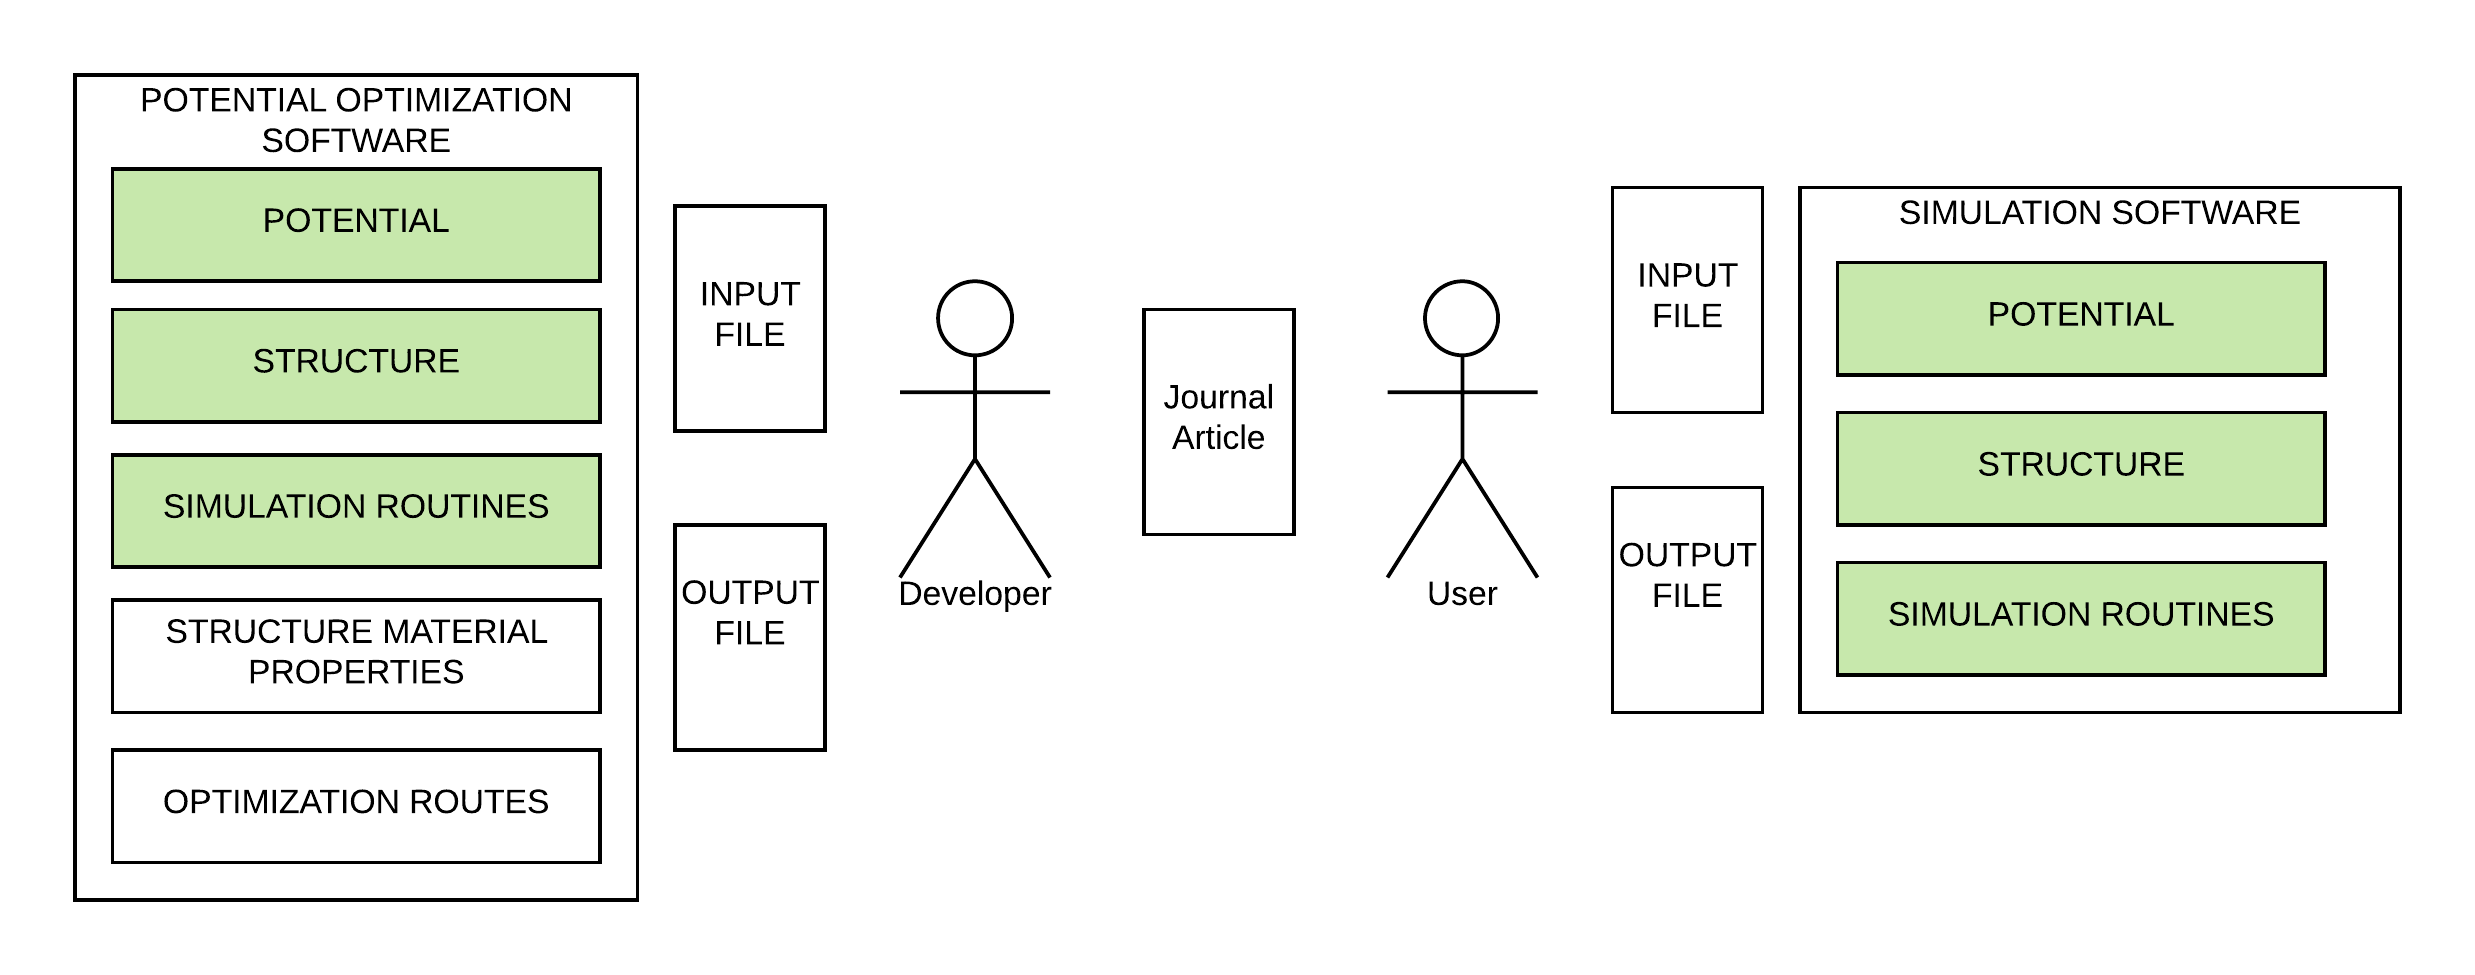
\includegraphics[width=5in]{chapter6/img/fig_potdev_monolithic}
	\caption{Schematic of monolithic potential development software}
\end{figure}

Figure \ref{fig:potdev_monolithic} is a schematic between potential development software, simulation software, the potential developer, and the potential user.  In this software architecture, The code for implementing the potential, the structures, and simulation routines common to molecular dynamics software.

Computational atomistic simulation involves software which have been developed in a variety of different languages, including but not exclusive to C/C++, and Fortran.  The combination of compiler optimization from strict variable types, well-vetted numerical libraries, and availability of parallelization libraries makes these langagues well-entrenched for the forseeable future.  The most popular atomistic simulation codes have matured over long-periods of time, with significant code contributions from the developers of potential formalisms enhancing the capabilities of the software.  For example, LAMMPS was originally written in Fortran, ported to C/C++.

Similarly, potential development software likewise developed iteratively, but with drastically different results.  Early potentials were developed using proprietary simulation codes which were augmented to describe the ability to describe the specific set of simulations to conduct required to optimize a specific set of simulations to calculate structure-property relationships.   In addition, numerical optimization routines to minimize a cost function as described in chapter \ref{ch:potential_development}.  Software codes included the ability to assign weights to the function to encode preferences and evolved to include global optimization techniques, such as simulated annealing\cite{kirkpatrick1983_simmulated_annealing} to deal with the local minima.

Despite the drastic expansion in the amount of formalisms and maturation of simulation codes, potential development software remains tailored to specific potentials and applications.  Potential software was written which support a small subset of potential formalisms.  For example, \emph{POSmat}\cite{martinez2016_posmat} supports the development of COMB potential and \emph{potfit}\cite{brommer2015_potfit} supports the development of embedded atom potentials (EAM).  On the other hand, GULP supports development of potentials based on a relatively small set of material properties.

The monolithic software development model is ill-suited for the demands of potential development.  As indicated in Figure \ref{fig:potdev_monolithic}, the regions in green represents a replication in development effort with simulation codes.  The implementation, maintenance, and updating of molecular dynamics code is non-trivial.  This effort is duplicated and better implemented in widely-adopted software codes such as LAMMPS.  More importantly,  there is little incentive for a third-parties to implement new potential formalism to monolithic software development codes.

Discussed in depth in chapter \ref{ch:potential_development}, the final parameterization on depends choices made by the potential developer; this means that the process by which a potential is developed is generally neither fully documented, nor reproducible.  Moreover, there is currently no objective method for evaluating the suitability of the function form of the atomic potential or determining if the final parameterization selected yields the best possible fit to the fitting database.  Current parameterization processes generally involve the minimization of a single scalar cost function, typically a weight sum of some measure of the predicted value, $\hat{q}_i(\bm{\theta})$ and the reference values of the specific material property $\hat{q}_i$.

As a result, the final parameterization depends on the many choices made by the potential developer; this means that the process by which a potential is developed is generally neither fully documented, nor reproducible.  Nevertheless, the process of potential development largely remains non-transparent and subjective,\cite{martinez2013_fitting,martinez2016_posmat} involving the repeated intervention of a skilled potential developer.\cite{brenner2000_fitting}
This leads to issues to problems with reproducibility in potential development as the selection of weights and initial conditions are largely not documented with the literature.
As a result, this knowledge is largely proprietary, remains concentrated in potential development groups, and software for potential development remain rudimentary tools developed by the specific needs of potential development groups.

In addition, parameter optimization is dependent upon numerical optimization techniques indicated in orange in Figure \ref{fig:potdev_monolithic}.  As described by Ghosh and Chakraborty \cite{ghosh2014_potdev_pareto}, the general problem of parameterization is a classic problem in the application of black box functions.  Cost function optimization techniques are unable to obtain compromise solutions which are Pareto efficient, but are occluded within a convex region of performance space.

\subsection{Goals of this Software}

Software for potential software development is by necessity a complicated piece of software which draws expertise from many disciplines for software development.

The goal of pypospack is to provide a software with a flexible software architectural library from which potential developers can quickly create their own potential optimziation software, by leveraging an object-orient software framework based upon a series of core packages, which deliver specific functionality to \emph{pypospack}.

\subsubsection{Ease of Development}
The targeted audience of \emph{pypospack} is a potential developer would this software package to parameterize ther own potentials using an existing formalism by modifying the existing examples distributed with this program.

In this case, the functional form of interest is already implemented in an external simulation code, but not implemented in \emph{pypospack}.  A goal of \emph{pypospack} is minimize the time spend in software development, so the potential spends more time in simulation and analysis of candidate potentials.

Ease of development is primary concern, computational efficiency is the secondary concern.
Rather than searching for computational efficiency by making \emph{pypospack} more monolithic, the design decision should instead prefer to leverage existing capability of external simulation codes.

Software for potential development is by necessity complicated.  The topic is technical requiring an understanding in doing computational simulations, combining these simulations to calculate material properties, then applying numerical analysis techniques to create candidate potentials.

The monolithic nature of existing potential optimization codes make code contribution difficult, because few people have the requisite expertise to understand all the implementation details in the code.

To break the problems of monolithic software development, \emph{pypospack} implements an object-oriented framework with extensive use of base classes to encapsulate implementation.  \emph{pypospack} decomposes the problem so that new functionality is focused on developing new code, rather than modifying existing code.  Additionally, since new functionality subclasses the base classes, any improvements in the computational efficiency or accuracy of either the base class or an encapsulated class improves the performance of contributed code as well.

\subsubsection{Scalability}

\emph{pypospack} should not only scale to use HPC asssets, but most components should be sufficiently lightweight so that development, testing, and analysis can be done on a personal workstation

In its primary use, the potential developer approximates the set of parameters  which produces Pareto optimal predictions, $\bm{\Theta}^*$.
In the process described in Chapter \ref{ch:methodology}, the space containing parameters, $\bm{\theta} \in \bm{\Theta}$, is sampled from a probability distribution, $\bm{\theta}(\omega) \in \bm{\Theta}(\Omega)$.
Many of the potentials evaluated will be non-optimal and converging of probability distributions from the initial distribution to the final distribution is slow.

To ameliorate this computational issue, \emph{pypospack} should be written to support different concurrency schemes.  \emph{pypospack} objects should be written to easily support serialization and deserialization, so that concurrency can be implemented through messaging passing technologies.

At the same time, it is important that \emph{pypospack} runs on workstations.  First, modern development is usually iterative and focuses on the implementation and testing of classes and methods.  A minimal amount of classes should be MPI-aware, parallelization code is notoriously difficult to test.
In modern data analysis processes, data analysis is interactive.  Configuration files and data files should be easily serializable to make interactive data analysis more accessible.
In support of this goal, \emph{pypospack} is implemented in Python which has strong support for interactive execution environments.  Large amounts of data are stored natively in popular data analysis frameworks.

\subsubsection{Flexibility}

\emph{pypospack} delivers a software library with a flexible architecure library.  From these components, applications for potential optimization and potential analysis should be able to developed quickly.  This should enable potential developers to tailor potential optimization software for their own needs.

Like other potential development software packages, \emph{pypospack} was developed to seprate the process of parameter optimization from the selection of the analytical form of the potental.  \emph{pypospack} separates itself from other packages by designed using object-oriented methods which enables users of this software to quickly implement potentials supported by external codes, calculate new material properties, and even replace the optimization techniques.

Despite the technical nature of the process, the process of potential development has a variety of decisions in the choice of material properties to optimize .  In addition, since empirical potentials are approximation of the potential energy surface, the potential selection is a value judgement, dependent upon the experience and skill of the potential developer.

The key driver of this software is to implement a systematic methodology to fit interatomic potentials that allows the objective evaluation of the quality of the parameterization, and the stability of the functional form, and that is both completely algorithmic and reproducible.

\subsubsection{Extensibility}

Likewise, this software has a functional requirement to explore issues regarding parametric uncertainty of interatomic potentials described by analytic functional forms.
This topic is very broad which includes the topic of multi-objective optimization, uncertainty quantification of predicted material properties propogated from uncertainty in the empirical potential's parameters, and the application of machine-learning techniques.
All these topics are active areas of research drawing interest from multiple-disciplines.  The \verb|pypospack| framework should likewise be flexible to quickly enable the implementation new algorithms and approaches toward this problem.

More generally, the secondary goal of this software project is to implement the necessary architecture for potential developers to write their own potential development software, either by extending the base the class to include more potential formalisms, simulations tasks, and calculation of material properties.  As a result, specific software architecture decisions were made to decouple the base classes from each other.

In general, this software focuses on the integration of other software.  It interacts with other software packages, but is loosely coupled by encapsulating interation of that software through an integration layer of objects.

In this way, it is possible to change the third party software dependencies by the implementation of a new integration layer.  Despite this loose coupling, great care was taken to ensure the selection of prominent softwre packages.  The benefits of using widely-accepted existing software include avoiding the mistakes involved from self-implementation, saving development effort, and that the underlying routines have sufficient documentation and support.


\subsection{Structure of this chapter}

This chapter starts by first discussing architectural considerations taken into account in the development of this software library.  Section \ref{sec:software_architecture} includes language selection, incorporation of prominent software packages, and core design choices which has implication for the use of this software package.  At the heart of the problem is the implementation of potentials, structures, and material properties which are described first.

Section \ref{sec:potential_evalaution} deals with the generalizing the calculation of material properties.  The calculation of material properties is often decomposed into several different simulations, the simulations executed, and the results gathered.  With the results from the individual components calculated, the material property of interest can then be calculated.  This section describes how this model decomposition is implemented and the execution framework evaluating a single parameter.

Both of these sections implements concepts introduced in Chapter \ref{ch:potential_development} and reuses the notation.  With the evaluation of a single parameter set accomplished, Section \ref{sec:software_sampling_strategies} describes implementation of the evolutionary strategy described in Chapter \ref{ch:methodology}.  In addition, to a discussion of the types of strategies implemented, this section specfically discusses how computational scalability is achieved by resolving concurrency and parallelization issues to ineable this software's use in high-performance computing environments.

While older monolithic codes have terse input and output files, the issues of accessibility to software in \emph{PyPOSPack} are resolved through the concept of object serialization and deserialization.  Section \ref{sec:softwre_acessibility} describes this strategy.  Since every object in \emph{PyPOSpack} can be instanced by a dictionary datastructure, the definition of an optimization process can be represented as a nested list of dictionaries.  This enables potential developers to define evolutionary strategies quite compactly, since the the deserialization results of the previous interation are used to serialized the next iteration.

Section \ref{sec:software_analysis}, we demonstrate the power of this framework, by looking at how the large amounts of data produced by simulation methodology is readily available to potential developer using well-known data analysis tools.  With the removal of traditional input and output files, the large amounts of data generated are readily accessible and accessible for exploratory data analysis.

\section{Software Architecture}
\label{sec:software_architecture}

\subsection{Licensing}

\subsection{Programming Language}
\emph{PyPOSPack} is written in Python 3 to leverage the strength of python as a high-level language for writing scientific applications.  Python has a liberal open source license which makes the distribution of the application without license issues.  Compatability across platforms is a major design consideration.  Since Python available of a wide variety of operating systems, there are few issues with portability as \emph{PyPOSPack} is written to be platform agnostic.

\emph{PyPOSPack} utilizes prominent open-source packages from the python community.  Python is popular programming language that is popular for scientific applications, due to the maturity and stability of fundamental numerical libraries, quality of documentation, and availability of well-supported distrbutions, such as Anaconda\cite{python_anaconda}, makes Python accessible and convenient for a broad audience.  Additionally, matplotlib\cite{hunter2007_matplotlib} integrated with IPython\cite{} provides an interactive research and development environment with data visualization suitable for most users.  As a result, is an appealing choice for algorithmic development and exploratory data analysis\cite{dubois2007_python}

\subsection{Integrated Software Packages}
Since, \emph{PyPOSPack} takes a different approach to the development of potentials by identifying a set of Pareto optimal potentials through an evolutionary process.  NumPy\cite{walt2011_numpy} adds an array language, similar in syntax to MATLAB, and similar in power to Fortran, in which operations are performed in compiled code.  This package provides linear algebra capabilities through this extended interfaces to BLAS\cite{blas2002} and LAPACK\cite{anderson1990_lapack}.  Scipy\cite{jones_scipy} builds on top of NumPy to provide functionality for optimization, numerical integration, and a statistics package for creating random variates.

The python language has a clean syntax yet has sophisticated constructs which allows is indifferent to either procedural or object-oriented programming styles, as the situation dicates.  Software development for this program was developed using procedural code, which was later encapsulated to classs object to abstract the implementation details into base objects.  The success of \emph{pymatgen} in transforming the high-throughput search of materials,  where the materials properties can be predicted by solving fundamental laws of physics using quantum mechanical appoximation such as density functional theory (DFT).  This virtual testing of materials was employed to design and optimize materials \emph{in silico}.

For the purposes of data analysis, the data produced by \emph|pypospack| is exposed through Pandas\cite{mckinney2010_pandas} to simplify data management and data analysis tasks using well known syntax.
Scikit-learn\cite{pedregosa2011_sklearn} integrates a wide range of machine learning algorithms for medium-scale supervised and unsupervised problems. This package focuses on bringing machine learning to non-specialists using a general-purpose high-level language.

Scalability for \emph{pypospack} is provided through the MPI for Python(mpi4py(\cite{dalcin2005_mpi4py,dalcin2008_mpi4py} which provides bindings of the Message Passing Interface (MPI)\cite{mpi2015} standard for the Python programming language and allows the exploitation of multiple processors in an HPC environment.  This is important for ease of installation and portability, as providing libraries around Fortran code can prove challenging on various platforms.

\subsection{Supported Simulation Codes}

The success of these approaches is largely driven by epistemic uncertainty associated with DFT calculations are largely driven by the unknown functional form of the exchange correlation functional.

Contrast this to molecular dynamics, where $V(\bm{r}_{ij})$ has uncertainty in both the functional form and parameterization.  Before attacking problems with functional form,

Let us first consider, three fairly simple systems which are widely studied, where the fundamental physics are significantly different.  Metal systems are described by
\emph{metal} units, where further information can be found in the LAMMPS

\subsection{Software Design Principles}

This software package is implemented in a way to minimize the mathematical and technical requirements for contributing to this project.

In the development of \emph{pypospack} the abstract base classes has been refactored many times as to encapsulate as much technical implementation into base objects as possible.  The base class objects encapsulates the run-time execution details.  As a result, the development of new classes to model to potential formalisms, simulation cells, simulation tasks, and the calculate material properties, can be developed with minimal effort.  If the material properties can be calculated using results from reference LAMMPS scripts with a rudimentary understanding of object-oriented programming and Python programming competence.

Since every implemented class in \emph{pypospack} is inherited from a base class, to develop a new subclass the appropriate the base class, the necessary methods required to be overidden are defined by a method signature, which by default generates a \verb|NotImplementedError|, if the functionality is required but not implemented.

A subclass which implements all the necessary features of a base class is referred to as an \emph{implemented class}.  A subclass which does not implement all the necessary features of a base class is a \emph{derived base class}.  In the \verb|potential| package, the \verb|PairPotential| is a derived base class because  it does not implement all the method required by the \verb|Potential| class.  However, it does define methods which encapsulates implementation details which are used for implemented pair potentials such as \verb|BuckinghamPotential|.

For example, classes which implement an empirical potential formalism are all subclasses of the \verb|Potential| base class.  The \verb|write_lammps_potential_section(filename)| method signature is constant across all subclasses and does not need to be implemented.
Instead, \verb|lammps_potential_section_to_string()| method needs to be overriden and returns the string variable required in the LAMMPS input file, which is used by \verb|write_lammps_potential_section(filename)|.
Here, the subclass inherits the \emph{specification} of the method \verb|lammps_potential_section_to_string| the details of the implementation are needed.  In constrast, the subclass inherits the \emph{implementation}  of \verb|write_lammps_potential_section| abstract class.
Here the disk output implementation is encapsulated in the base class, and the potential developer is not concerned about integrating this new class into the existing code base, other than their implemented methods produce the required behavior.
This software architecture approach makes code development for \emph{pypospack} less intimidating since the more difficult implementation details have encapsulated within the base classes.

Each implemented class is required to implement certain static variables.  For example, every implemented \verb|PairPotential| class, is required to provide a unique the static string \verb|potential_type_id| and \verb|pair_parameter_names|.  This enables code introspection, the ability of \emph{pypospack} to examine its own classes.  As a result, new functionality only requires its implementation in a new file, place it in the correct subpackage directory, and \emph{pypospack}'s introspection code will automatically integrate it into the application.

Due to the complexity of these classes, all classes have usually simple constructors, requiring only minimal information required for instantiation, compared to other workflow projects such as \emph{pymatgen}.  This design decision in intentional.  Within this software library class instantiation, class configuration, and class execution are intentionally decoupled in the base classes.  By keeping class instantiation simple, the base classes from being brittle.  If abstract classes are tightly coupled to a small set of use cases, then the abstract class is described as brittle when new use cases are unable to reuse either the specification or implementation of a base class.  As \emph{pypospack} is designed to accomodate a wide variety of potential formalisms, simulation tasks, and material properties, classes within \emph{pypospack} are designed to be as general as possible.

To specialize subclasses for more specialized purposes, configuration of objects are done after class initialization by passing dictionaries into methods.  Every object within \emph{pypospack} can initialized and configured by dictionary initializtion.  Known more generally as a hashtable, these collections of key-value pairs are implemented in Python as a data structure called a dictionary (i.e. \verb|dict| or \verb|OrderedDict|).
  Since method specification is generalized, it is easier to encapsulate dozens of different classe representing potentials, simulations tasks, and material properties, without requiring the implementation of specific \emph{if}-\emph{else if}-\emph{else} idiomatic expressions, which must be rewritten every time new functionality is added to \emph{pypospack}

Since dictionaries are used for initialization, \emph{pypospack} makes extensive use of object serialization, by encapsulating pertinent information into a data structure of key-value pairs.
The implementation of the dictionary constructor has the benefit of providing object serialization from strings.  PyPOSPack implements YAML("YAML Ain't Markup Language")\cite{yaml_version_1_2r} object serialization as a compromise between XML ("eXtensible Markup Language") and the definition of their schemas and JSON ("JavaScript Object Notation").  These three file format have prominent existing libraries, which prevents mistakes which can occur from implementing file parsers
One problem with potential development software are system integration issues involving the creation of input files and parsing of output files.

The currently implemented classes have straight forward implementations, well-documented, and provide templates to encourage others to contribute to the \emph{pypospack} software.

\subsection{Potential Formalisms}

The software development effort associated with developing new potentials for potential optimization software is typically time-consuming, requiring the implementation not only of the potential $\hat{V}$ but also the implementation of the second-derivatives with respect to changes in interatomic positions to computational issues with numerical approximation.  In \emph{PyPOSPack}, this requirement has already been implemented by the simulation software, which drastically reduces the software development time to implement existing formalisms already supported by either LAMMPS or GULP.

The \verb|potential| package contains class objects which inherit from the appropriate abstract base class and overide the required methods for implementation.  The \verb|Potential| abstract class only expects implementation of the \verb|_init_parameter_names|, \verb|lammps_potential_section_to_string|, \verb|gulp_potential_section_to_string|, \verb|lammps_parameter_file_to_string| and \verb|evaluate| methods.  However, not each method needs to be implemented.

Depending upon the use of the potential, not all methods need to be overridden.  For example, if simuations are only run in LAMMPS, then the only the \verb|lammps_potential_section_to_string| would need to be implemented to be implemented respectively.

Likewise, some implemented \verb|Potential| classes are not implemented in LAMMPS or GULP and are used in the composition of tabulated values.  In these cases, only the \verb|evaluate| method is required to be implemented.

In \emph{PyPOSPack}, the \verb|potential| package contains classs objects, which inherit from methods from the appropriate base class.  The base classes have been implemented in \verb|potential|: (1) \verb|PairPotential|, (2) \verb|ThreeBodyPotential|, (3) \verb|EamDensityFunction|, and (4) \verb|EamEmbeddingFunction|.
\subsubsection{PairPotential}

In \emph{pypospack} applications, a potential formalism is defined by specifying the \verb|potential_type| and the \verb|symbols| as an dictionary object:
\begin{lstlisting}[language=Python]
potential_formalism = OrderedDict()
potential_formalism['potential_type'] = 'buckingham'
potential_formalism['symbols'] = ['Mg','O']
\end{lstlisting}

The \verb|PairPotential| implements a standard potential naming scheme.  As a result, it is necessary only to define the \verb|pair_parameter_names| attribute in implemented potential classes.  For example, for a pair potential with a parameter, $A_{Mg,O}$, satifies the $A$ parameter of the Mg-O pair potential term, and would have the name \verb|MgO_A|.  The recommended convention for naming parameters is to prefer the same variable naming convention scheme listed in LAMMPS documentation, then the variable naming scheme listed in original literature.

To evaluate a specific potential the parameter set must be defined as a dictionary object.  For example, as part of a collection of reference potentials, the dictionary object containing the original parameterization is
\begin{lstlisting}[language=Python]
reference_potentials['SW'] = OrderedDict([
    ('SiSiSi_epsilon',2.1686),
    ('SiSiSi_sigma',2.0951),
    ('SiSiSi_a',1.80),
    ('SiSiSi_lambda',21.0),
    ('SiSiSi_gamma',1.20),
    ('SiSiSi_costheta0',-1/3),
    ('SiSiSi_A',7.049556277),
    ('SiSiSi_B',0.6022245584),
    ('SiSiSi_p',4.0),
    ('SiSiSi_q',0.0),
    ('SiSiSi_tol',0.0)
])
\end{lstlisting}

Implemented pair potentials are indicated in Table \ref{tbl:pypospack_pair_potential}.

\begin{table}[ht]
    \centering
    \caption{Implemented pair potentials in \emph{PyPOSPack}.}
    \label{tbl:pypospack_pair_potential}
    \begin{tabular}{ccccc}
	    \hline
	    {Class Name} & LAMMPS & GULP & EAM  & {Reference} \\
	    \hline
	    BuckinghamPotential   &   &   & x & \cite{lewis1985_buckingham,buckingham1938} \\
	    MorsePotential        & x & x & x & \cite{morse1929_morse_potential} \\
	    BornMayerPotential    &   &   & x & \cite{abrahamson1969_bornmayer_potential} \\
	    LennardJonesPotential & x & x & x & \cite{lennardjones1924_lj_pot} \\
	    GeneralizedLennardJonesPotential
	                          &   &   & x & \cite{mishin2004_eam_NiAl} \\
	    \hline
    \end{tabular}
\end{table}

\subsubsection{Three Body Potentials}
Three body potentials are implemented in with the base class \verb|ThreeBodyPotential|, and listed in Table \ref{tbl:pypospack_threebody_potentials}.  Unlike pair-potentials, the potential naming schemes are not equivalent.

In the Stillinger-Weber potential\cite{stillinger1985_sw}, a pair potential term $V_2(r_{ij})$ is dependent upon the interatomic separation distance between atoms $r_{ij}$ between atoms $i$ and $j$.
To model angular dependence the three-body term $V_3(r_{ij},r_{ik},\theta_{ijk})$ augments the $V_2$ term, where $i$ is the central atom in a three body interaction.  In a Stillinger-Weber potential, an entry for \verb|SiSiC| and \verb|SiCSi| are identical since \verb|Si| is the same.

In comparison, the Tersoff potential\cite{tersoff1988_tersoff} is a pair interaction term describing the bonding of atoms $i$ and $j$ influenced by the presence by a third atom $j$.
In the Tersoff potential, an entry for \verb|SiCC| means that a silicon atom is bonded to a carbon atom and influenced by a third atom.  The three-body parameters for \verb|SiCC| and \verb|SiSiC| are not necessarily the same.  As a result, \verb|_init_parameter_names| has different implementations for three-body potentials, and the base class has not default implementation.

\begin{table}[ht]
	\centering
	\caption{Implemented three-body potentials.}
	\label{tbl:pypospack_threebody_potentials}
	\begin{tabular}{cccc}
		\hline
		{Class Name} & LAMMPS & GULP & Reference \\
		\hline
		TersoffPotential & x & x & \cite{tersoff1988_tersoff} \\
		StillingerWeberPotential & x & x &\cite{stillinger1985_sw} \\
		\hline
	\end{tabular}
\end{table}

\subsubsection{EAM Potentials}

The formalism of the EAM potential is composed of three functions: (1) a pair potential, (2) an electron density function, and (3) an embedding energy function which is dependent upon individual contributions defined by the electron density function.
The implementation of the \verb|EamPotential| class encasulates a \verb|PairPotential|, a \verb|EamEmbeddingFunction|, and a \verb|EamDensityFunction|.

  A density function $\bar{\rho}(r_{ij})$ is the electron density contribution of atom $j$ to the total electron density at the site for atom $i$.  Like a pair potentia, it is a function the interatomic separation distance.  However, each species is bound to an electron density function.  For an EAM potential with two chemical species, there are two electron density functions.  Thus the parameter naming convention would be \verb|{symbol_1}_{parameter_name}|.
	The list of implemented EAM density functions are listed in Tables \ref{pypospack_eam_density_function}.

\begin{table}[ht]
	\centering
	\caption{Implemented EAM density functions}
	\begin{tabular}{cc}
		\hline
		{Class Name} & {Reference} \\
		\hline
		ExponentialDensityFunction & \\
		Mishin2004DensityFunction & \cite{mishin2004_eam_NiAl} \\
		\hline
	\end{tabular}{cc}
\end{table}

An energy embedding function, $F(\bar{rho}_i)$, calculates the energy required to embed atom $i$ based upon electron density at the site.  Like the EAM density function, the embedding function is defined for each chemical species and has a similar naming convention for its parameters.
\emph{pypospack} supports two representations of the embedding function.
The default implementation defines the embedding function, $F(\bar{\rho}|\bm{\theta})$, as regular analytical function.

The second representation comes from determing the embedding function implied by the equation of state, a technique pioneered by Foiles \emph{et al.}\cite{foiles1986_eam_embedded_eos}.
The \verb|EamEmbeddingEquationOfState| provides a base class for the numerical estimation of these functions, and are listed in Table \ref{tbl:pypospack_eos_embedding_function}.
Although not typically included in the definition of the parameter set, a string variable specifying host lattice (e.g. fcc, bcc, hcp) of the ground state, \verb|lattice_type|, as well as the lattice parameter, $a_0$ are necessary.

\begin{table}[ht]
	\centering
	\caption{Implemented Analytical embedded energy function.}
	\label{tbl:pypospack_embedding_function}
	\begin{tabular}{cc}
		\hline
		{Class Name} & Reference \\
		\hline
		BjsEmbeddingFunction & \\
		UniversalEmbeddingFunction & \\
		FinnisSinclairEmbeddingFunction & \\
		\hline
	\end{tabular}
\end{table}

EAM potentials are not defined in simulation software as analytical potentials, but provided in a pre-calculated tabulated the \emph{setfl} format.  The class \verb|SetflFile| contained in the \verb|eamtools| packages deserializes a parameterized EAM potential into the expected format.

\begin{table}[ht]
	\centering
	\caption{Implemented EAM embedding function determined from the inverse equation of state}
	\label{tbl:pypospack_eos_embedding_function}
	\begin{tabular}{cc}
		\hline
		{Class Name} & {Reference} \\
		\hline
		RoseEosEmbeddingFunction & \cite{foiles1984_eam_eos} \\
		ZopeMishinEosEmbeddingFunction & \cite{zope2003_eam_eos} \\
		\hline
	\end{tabular}
\end{table}

To define an EAM potential, it only necessary to specify the chemical species, and the formalism of the pair, density, and embedding function.
\begin{lstlisting}[language=Python]
	potential_formalism = OrderedDict()
	potential_formalism['potential_type'] = 'eam'
	potential_formalism['symbols'] = ['Ni']
	potential_formalism['setfl_filename'] = None
	potential_formalism['pair_type'] = 'bornmayer'
	potential_formalism['density_type'] = 'eam_dens_exp'
	potential_formalism['embedding_type'] = 'eam_embed_eos_rose'
\end{lstlisting}

\subsection{Structural Representation}
\label{sec:pypospack_structures}

The representation of a structure was formalized in Section \ref{sec:configuration_space}, but impose certain restrictions to communicate information on about the unit cell, and ensure that geometry is compatible with LAMMPS.
The lattice vectors of a simulation cell are embedded in Euclidean space,  $\bm{a}_i = [a_{11}, a_{12}, a_{13}] \in \mathbb{R}^3$ for $i \in [1,2,3]$.  To ensure that the crystal structure can be defined in LAMMPS, we impose restructions defined by the following matrix representation:
\begin{equation}
	\begin{bmatrix}
		a_{11} & a_{12} & a_{13} \\
		a_{21} & a_{22} & a_{23} \\
		a_{31} & a_{32} & a_{33}
	\end{bmatrix}
	=
	\begin{bmatrix}
		\ell_x    & 0         & 0     \\
		\tau_{xy} & \ell_y    & 0     \\
		\tau_{xz} & \tau_{yz} & \ell_z
	\end{bmatrix}
\end{equation}
Here $\ell_x$, $\ell_y$, $\ell_z$ define a length of parallelpiped unit in the orthogonal $\hat{u}_x$, $\hat{u}_y$, and $\hat{u}_z$ directions with $\tau_{xy}$, $\tau_{xz}$, and $\tau_{yz}$ representing how much the parallelpiped is tilted from the orthogonal axis.

For a unit cell, the magnitude of the lattice vectors $\bm{a}_1$, $\bm{a}_2$, and $\bm{a}_3$ correspond to the $a$,  $b$, and $c$ from the typical crystallographic representation of a unit cell.  In order to encode this information, each $\bm{a}_i$ is normalized by transforming $\bm{a}_1$ unto a unit vector by its length $a_0$.  For a cubic system, the matrix representation now becomes
\begin{equation}
\label{eq:pypospack_lattice_vector}
	\begin{bmatrix}
		a & 0 & 0 \\
		0 & b & 0 \\
		0 & 0 & c
	\end{bmatrix}
	=
	a_0
	\begin{bmatrix}
		1 & 0 & 0 \\
		0 & \frac{b}{a} & 0 \\
		0 & 0 & \frac{c}{a}
	\end{bmatrix}
	=
	a_0 \begin{bmatrix}
				\bm{h}_1 \\
				\bm{h}_2 \\
				\bm{h}_3
			\end{bmatrix}
	=
	a_0 \bm{H}
\end{equation}

To represent a supercell $n_1 \times n_2 \times n_3$, the modified $\bm{H}$ matrix then becomes
\begin{equation}
\label{eq:pypospack_supercell_representation}
	a_0 \bm{H}'
	=
	a_0 \begin{bmatrix}
	        n_1 \bm{h}_1 \\
					n_2 \bm{h}_2 \\
					n_3 \bm{h}_3
			\end{bmatrix}.
\end{equation}

Representations of crystal structures is implemented in the package \verb|crystal|.  The base class for all crystal structures is \verb|SimulationCell|.  Representation of the lattice vector is set by determining Equation \ref{eq:pypospack_lattice_vector}, by setting the attribute values \verb|a_0| and \verb|H|, where \verb|H| is a $3 \times 3$ matrix stored as a \verb|numpy.ndarray|.  The \verb|atomic_basis| attribute is a \verb|list| of \verb|crystal.Atom| objects which store in addition to the position $\bm{r}$, the chemical species $\alpha$, and a variety of optional \verb|None| assigned attributes which can be assigned to represent physical quantities such as charge and magnetic moment.  A number of optional convenience methods and factory functions, such as getting the number of atoms of each chemical species are represented, creating supercells, and adding/removal of atoms to point defects.

For intercompatibility with the VASP file format for structures, \verb|io.vasp.Poscar| is a subclass. \verb|SimulationCell|.  This class can read and write POSCAR formatted files through the implemented \verb|read()| aand \verb|write()| methods.
To interact with LAMMPS has likewise been created in \verb|io.lammps.LammpsStructureFile| object through the \verb|io.gulp.get_structure_string()| and \verb|write()| methods
Access to the tools to create orthogonal cells from hexagonal lattices and provide different orientations of the lattice is automated through integration of the Atomic Simulation Environment (ASE)\cite{larsen2017_ase}.

The creation of a structure database is defined by class \verb|StructureDatabase|.  The structure database has two important attributes consisting of a \verb|path| attribute variable which contains the path to the directory containing all the structures.  For each structure, one needs to provide the \verb|filename| of the structure file and a unique string which serves as the key value to identify the structure.  Examples contained within the \verb|pypospack| distribution, use the chemical composition, the crystal structure, and the type of crystal structure.  For example, a representative FCC unit cell of nickel would be referred to by \verb|Ni_fcc_unit|.

The creation of structure files is often one of the more challenging processes for someone new to computational materials science.  To aid in the creation of a structure database, a variety of convenience classes and factory methods help automate the instantiation of these objects, identity points where interstitial defects can be inserted, orient crystals to common miller index locatations, create slabs for surface calculations, reciprocal space lattice vector, and get $k$-point paths for bandwidth calculations.  Currently, this functionality is implemented for face centered cubic, $\alpha$-quartz, diamond cubic, and rocksalt crystals.

\section{Modelling and Execution Framework}
\label{sec:potential_evalaution}

At this point, the discussion moves to the fundamental functionality, which automates a set of material properties for a given functional form for a variety of parameters.  Since one of the goals of this software package framework is to provide a lightweight modelling framework, which encapsulates implementation details within abstract classes.

Unlike \emph{ab initio} DFT automation frameworks which conducts a simulation for permutations of a structure in search for an optimal material.  Each calculation here is expensive, requiring tens of minutes or even hours of simulation per calculation.  Here we have a smaller number of structures, which remain fixed while we iterate over a large number of calculations which take a short amount of time.  As a result, the engine to manage the workflow is much different.

This section first with a discussion of a modelling workflow for the calculation of material properties, by going through the process of automating the defect formation energy.

\subsection{Modeling Framework}

To run simulations, \emph{pypospack} spawns a new process, through the Python \verb|subprocess| module, and obtain the exit codes, which is returned from the child process and is interpreted by \verb|pypospack| in the event of external codes returning a success or failure.  Through this facility, input files are made for the external executable, which is run under a child subprocess until an exit code is detected, when the output files of the energy calculator are then parsed for pertinent information.  Currently, \verb|pypospack| supports LAMMPS, GULP, VASP as external energy calculators.  The VASP functionality is not fully featured and exists to promote consistency in the calculation of \emph{ab initio} reference values $\bm{q}$.

The choice to use an external energy calculator rather than implementing one internally was chosen to eliminate the maintenance of simulation software and implementation of potential formalisms.  Even for potential developers who create new functional forms, code design, implementation, and maintenance is limited to their code code contributions in LAMMPS.
While an application programming interface (API) to LAMMPS does exist, \emph{pypospack} implements the calculation of material properties through input and output files is a practical necessity.  Computational materials scientists already have existing LAMMPS scripts which are reused for compute a variety of material science properties.  Using a "process determines software design" approach, an approach for the automation of material properties is now presented.

To demonstrate the ability of this framework to quickly automate the calculation of material properties, the process for the automation of a point defect calculation is demonstrated.

\begin{figure}[ht]
	\label{fig_point_defect_calculation}
	\centering
	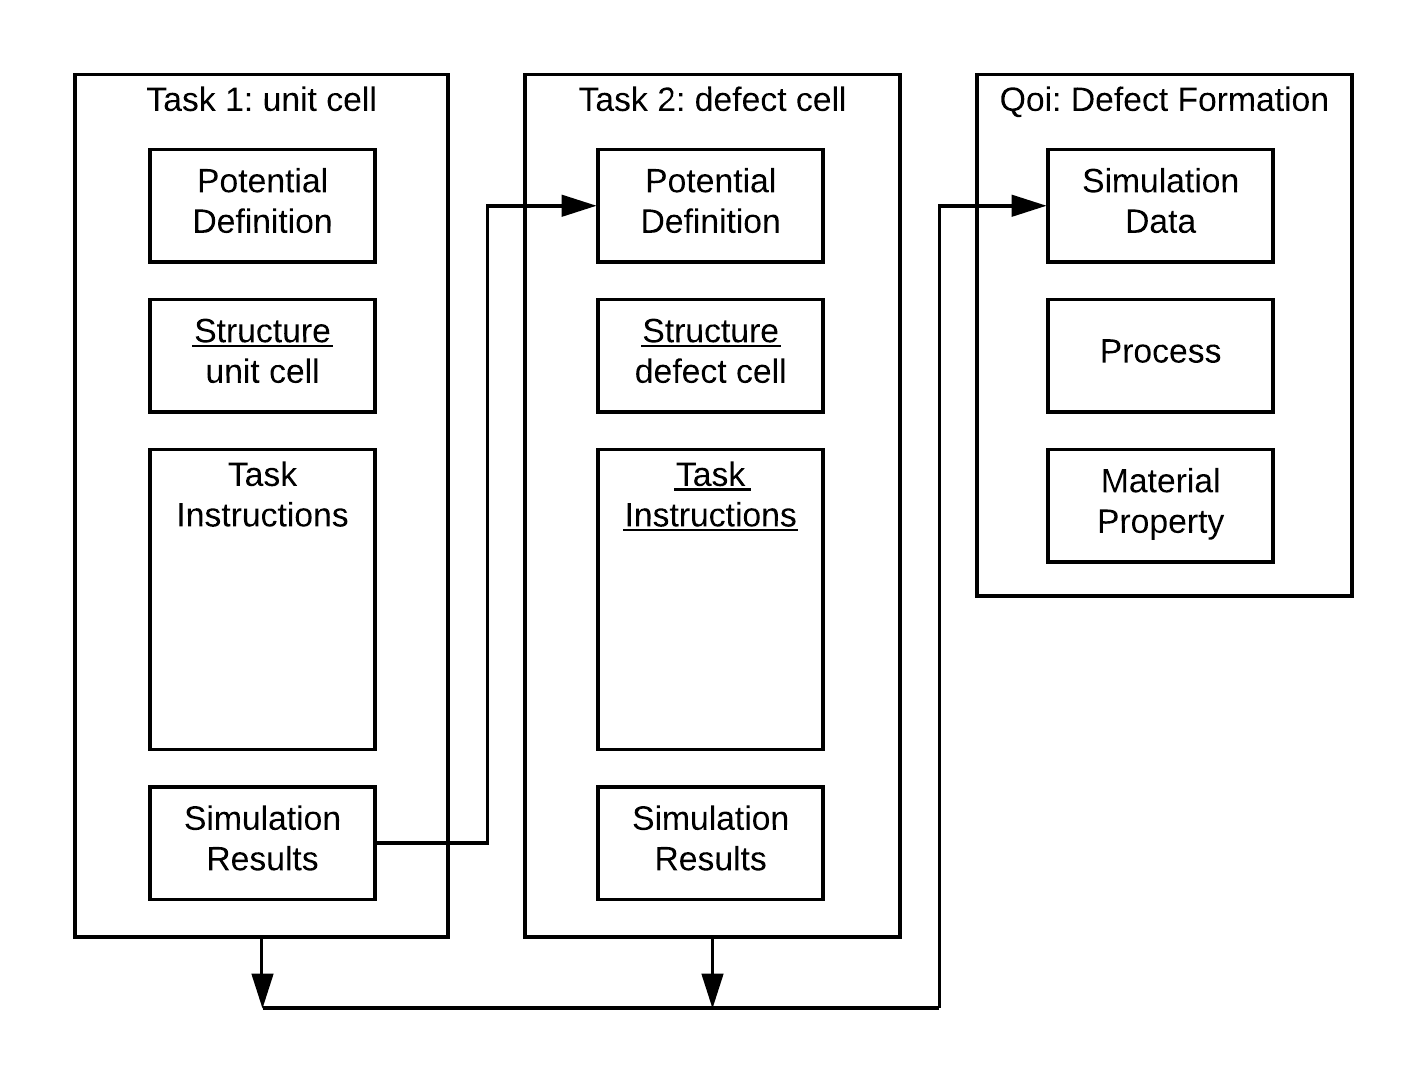
\includegraphics[width=5in]{chapter6/img/fig_point_defect}
	\caption{Schematic of for the calculation of point defect calculations.}
\end{figure}

In the first step of the automation process, a potential developer first creates a set of reference simulations required to calculate a material property.  Figure \ref{fig_point_defect_calculation} provides a schematic of various components involved in the calculation of a quantity of interest using the supercell method.  In this case, it starts at a series of LAMMPS or GULP scripts, with the calculation of the material property done with a commercial spreadsheet calculations.

\subsubsection{Simulation Tasks}

In \emph{pypospack}, the execution of simulation tasks are subclasses of \verb|Task| class.  The derived base classes \verb|LammpsTask| and \verb|GulpTask|, provides the necessary methods for implementing LAMMPS and GULP simulations. \verb|Task| objects are primarily responsible for managing the input and output files for simulation against an external code.  In the expected use of these classes for parameter optimization, external simulation are run a subprocess to a \emph{pypospack} application, and derived base classes are reponsible for managing these subprocesses.

In the case of LAMMPS simulations, the simulation scripts consists of four sections:  the potential definition, the structure definition, instructions to calculate the required simulation, and an output section.  GULP input scripts are decomposed in a similar way.

 This class encapsulates the \verb|Potential| class and the \verb|SimulationCell| class.  As a result, to implement a \verb|Task| class requires three steps: (1) defining of LAMMPS instructions, (2) parsing the output file to retreive the results of the simulation, and (3) populate the \verb|task_results| dictionary with the results.  The first step is already completed in the reference LAMMPS script; the other two steps are rudimentary programming tasks.

The calculation of the Figure \ref{fig_point_defect_calculation} shows material property requires two simulations.  The first simulation involves one involving the minimization of a unit cell representing an ideal bulk structure.  In this simulation, a simulation process known as structural and position relaxation is conducted.  Here, the minimum energy basin is attains by either steepest descent or conjugate gradient method of minimizing the energy with respect to the atomic positions of each atom, the volume of the simulation cell, and the shape of the supercell.  This simulation provides the energy $E_{c,\mathrm{bulk}}$, as well as structural properties of the lowest energy atomic configuration of the phase represented by the unit cell.  This simulation type has been implemented in as \verb|LammpsStructuralMinimization| and has the \verb|task_type_id| of \verb|min_all|.

The second calculation a simulation involving a defect structure.  Here the defect is embedded into a larger supercell representation of the bulk structure.  This is necessary to prevent defect from interacting with itself across the periodic boundary conditions.  Here the shape and volume of the simulation cell is held fixed, while the conjugate gradient method minimizes the positions only.  This simulation type has been implemented in \verb|LammpsPositionMinimization| and has the \verb|task_type_id| of \verb|min_pos|.

A feature of this simulation workflow is that that running the defect calculation is dependent upon the structural properties of the of the ideal bulk system.  \emph{pypospack} solves this problem by aggregating the results of each results of each task into a dictionary object.  Each simulation task is assigned a unique \verb|task_id| which is determined by concatenation of the \verb|structure_id|, \verb|task_type_id|.  For example, if this simulation was done to calculate the vacancy formation energy of silicon, the bulk unit cell might have the name \verb|Si_dia_unit| and the defect structure \verb|Si_dia_vac|.  Then associated \verb|task_ids| would be \verb|Si_dia_unit.min_all| for the minimization of the ideal crystal structure and \verb|Si_dia_vac.min_pos| for the energy calculation of the structure containing the defect.

In the use cases encountered so far, simulations tasks are dependent upon the structural results of their associated bulk structure.  If the \verb|bulk_structure_name| attribute is set on a \verb|Task|, the class will modify the encapsulated \verb|SimulationCell| object to extract the lattice vectors from the associated structural minimization simulation.  If other dependencies are necessary, a new simulation task can be created by subclassing the \verb|LammpsTask| and implement the desired behavior using implemented existing classes as a template.

A simulation task may produce one or more values of intererst.  The simulation produces the cohesive energy $E_c$, and the lattice vectors $\bm{a}_1$, $\bm{a}_1$, and $\bm{a}_3$ of the relaxed structure.  Currently, \emph{pypospack} marshals all simulation results into a dictionary consisting of primitive data types.  As a result, components of the lattice vector $\bm{a}_1$, would have a key values of \verb|a_11|, \verb|a_12|, and \verb|a_13|.

A list of the all the simulation tasks, and a short descriptions are summarized in Table \ref{tbl:pypospack_tasks}.  All simulation task classes are derived from the  \verb|Task| base class. There are two derived base classes: \verb|LammpsTask| and \verb|GulpTask|.

\begin{table}[ht]
	\centering
	\caption{A list of the simulation tasks currently implemented in \emph{pypospack}.}
	\label{tbl:pypospack_tasks}
	\begin{tabular}{ccc}
		\hline
		\verb|task_type_id|
		& Class Name
		& Simulation Engine \\
		\hline
    \verb|min_all|
		& LammpsStructuralMinimization
		& LAMMPS
		\\
		\verb|min_pos|
		& LammpsPositionMinimization
    & LAMMPS
		\\
		\verb|min_none|
		& LammpsStaticCalculation
    & LAMMPS
		\\
		\verb|elastic|,
		& LammpsElasticCalculation
		& LAMMPS
		\\
    \verb|npt|,
		& LammpsNptSimulation
		& LAMMPS
		\\
		\verb|nvt|,
		& LammpsNvtSimulation
		& LAMMPS
		\\
    \verb|gulp_gamma_phonon|
		& GulpGammaPointPhonons
		& GULP
		\\
		\hline
	\end{tabular}
\end{table}

The execution structure for a \verb|Task| happens in stages to accomodate to modify the conditions of the simulation based on the results of other simulation.  The stages are encoded in the attribute \verb|status|.  The states a \verb|Task| listed in increasing progression: INIT, CONFIG, READY, RUNNING, POST, and FINISHED.  An additional state, ERROR, indicates when there is a problem with the simulation.  Likewise, each status has associated callback methods: \verb|on_INIT|, \verb|on_CONFIG|, \verb|on_READY|, \verb|on_RUNNING|, \verb|on_POST|, AND \verb|on_FINISHED|.  The callback methods can be overridden, but the callback argument signature cannot be changed.  This allows an external procedure to interrogate the status of a class, and then provide the necessary information to the class.

This software design has a specific purpose to support multiple \Tasks| initialized within a container such as a \verb|list| or \verb|dict|.  The tasks are monitored within a callback loop external to the \verb|Task| objects.  The callback methods of the \verb|Task| objects should be non-blocking so the thread running callback loop can continue to monitor all the simulation tasks.  While \emph{pypospack} is not multi-threaded, multiple simulations are run simulatenously per processor, since external simulation codes are run in a child subprocess forked from the \emph{pypospack} process.  The callback loop continues until all \verb|Tasks| have either reached a FINISHED or ERROR status.

When an instance of a \verb|Task| is created, the \verb|status| is set to INIT.  A simulation directory with a unique name is created to segregate the file system context of different simulations.  Since external code execution uses an input/output file strategy, it is necessary to provide a unique context to prevent filename conflict of concurrently running simulations.

The \verb|on_INIT| callback method provides either dictionary necessary to initialize a \verb|Potential| object or an existing \verb|Potential| object is passed by reference.  The secondary mechanism is used to eliminate the computational costs of tabulation of EAM potentials, which can be expensive when the embedding function is determined from inverting an equation of state.  When this task is completed, the \verb|status| attribute is changed from INIT to CONFIG.

the \verb|on_CONFIG| callback method allows the callback loop to provide information which is not available until another simulation is complete.  The results of all completed simulations are passed as a nested dictionary of simulations.  Since each \verb|Task| instance has a unique \verb|task_id|, the task processes the dictionary to identify determine the desired configuration for the simulation.  In our example, the defect calculation awaits the results of the structural relaxation calculation of the bulk system.  If the information is not possible, the \verb|status| attribute remains in the INIT state.  When all the necessary configuration information has been acquired, all the necessary input files are written to its simulation directory, and the \verb|status| attribute is changed from CONFIG to READY.

The \verb|on_READY| method encapsulates the \verb|run()| method.  The purpose of this encapsulation is to support multiple methods of task execution.  Support for serial execution of a \verb|Task| is implemented in the \verb|run()| method.  The method identified the location of the external simulation code from the operating system environment variables.  For LAMMPS, the environment variable is \verb|LAMMPS_SERIAL_BIN|.  For GULP, the environment variable is \verb|GULP_SERIAL_BIN|.  These implementation details are encapsulated in the \verb|LammpsTask| and \verb|GulpTask|.  The execution context is changed to its simulation directory, a non-blocking subprocess is created to run the external simulation code, using the Python \verb|subprocess| module to monitor the subprocess.  Some MPI environments, have a default configuration preventing a program from spawn a subprocess, but this can normally be disabled by setting the appropriate MPI environment available in the submission script.  Once the subprocess is created, the \verb|status| attribute is change from READY to RUNNING.

However, some \verb|Tasks| require MPI support such as NEB calculations.  Other simulations require parallelization in order to complete the simulations in a reasonable amount of time,  NPT and NVT molecular dynamic simulations requiring time integrations are examples.
Since \emph{pypospack} is an MPI-aware application, it is not possible for \emph{pypospack} to subprocess MPI-aware code.  In these cases, the execution of the task is responsibility of an HPC job submission manager, like \emph{pymatgen} implements.  \emph{pypospack} does not implement a persistence model for long-running simulations, but the examples to calculate material properties which are dependent upon long-running simulations is provided in the distribution.

The \verb|on_RUNNING| polls the external simulation code.  Here there are a variety of techniques used to identify a simulation failure.  First, the \verb|subprocess| module allows us to check is the application is running, exited normally, or exited with an error.  If the external simulation code, exited with an error, then the attribute \verb|status| is marked ERROR.    If the application is running, the \verb|Task| will check to see how long the simulation is running, if the total time of the simulation exceeds \verb|max_simulation_time|, a variety of process management steps are applied to kill the child process without interrupting the parent process.  If the simulation code exited normally, the attribute \verb|status| is marked POST, indicating the simulation is complete.

The \verb|on_POST| method instructs the task to parse the output files from the external simulation code and populate a dictionary containing the results of the simulation.  The attributes of the simulation both returned to the callback thread and set as the attribute value \verb|results|.  After the post-simulation activities have been completed, the \verb|status| attribute is sent to FINISHED.

This approach to software development allows contribution for other to contribute to developing \emph{pypospack}'s capabilities by developing new simulation tasks and calculation of material properties without requiring implementation of the interfering with the technical implementation.

\subsubsection{Material Properties}

The material properties is referred to more generally in the software by the term quantity of interest (QOI), a term coming from  from verification, validation, and uncertainty quantification (VVUQ) literature.
The calculation of material properties is implemented as subclasses of the \verb|Qoi| base class.

A Qoi class may implement the calculation of one or more material properties.



In writing the QOI class, it is desireable
The calculation of the Figure \ref{fig_point_defect_calculation} material property consists of two tasks.

\begin{table}[ht]
	\centering
	\caption{A list of the Qoi classes}
	\begin{tabular}{cc}
		\hline
		Name
		  & Description \\
		\hline
    GulpOptiCalculations
		   & \verb|gulp_opti_calc| \\
		StaticStructureCalculations
		   & \verb|lmps_min_none| \\
		RelaxedPositionCalculations
		   & \verb|lmps_min_pos| \\
		RelaxedStructureCalculations
		   & \verb|lmps_min_all| \\
    ElasticPropertyCalculations
		   & \verb|lmps_elastic| \\
		PhaseOrderCalculation
		   & \verb|phase_order| \\
		DefectFormationEnergy
		   & \verb|lmps_defect| \\
		SurfaceEnergyCalculation
		   & \verb|lmps_surface_energy|  \\
		StackingFaultEnergyCalculation
			 & \verb|lmps_stacking_fault| \\
		ThermalExpansion
			 & \verb|lmps_thermal_expansion| \\
		\hline
	\end{tabular}
\end{table}

\begin{table}[ht]
	\centering
	\caption{GulpOptiCalculations}
	\begin{tabular}{cc}
		\hline
		QOI name & description \\
		\hline
		\verb|Ecoh_min_all_g| \\
    \verb|a11_min_all_g| \\
	  \verb|a12_min_all_g| \\
	  \verb|a13_min_all_g| \\
    \verb|a21_min_all_g| \\
	  \verb|a22_min_all_g| \\
	  \verb|a23_min_all_g| \\
    \verb|a31_min_all_g| \\
	  \verb|a32_min_all_g| \\
	  \verb|a33_min_all_g| \\
		\hline
	\end{tabular}
\end{table}

\begin{table}[ht]
	\centering
	\caption{StaticStructureCalculations}
	\begin{tabular}{cc}
		\hline
		QOI name & description \\
		\hline
	  \verb|Ecoh_min_none|  \\
    \verb|a1_min_none|  \\
		\verb|a2_min_none|  \\
		\verb|a3_min_none|  \\
    \verb|a11_min_none|  \\
		\verb|a12_min_none|  \\
		\verb|a13_min_none|  \\
    \verb|a21_min_none|  \\
		\verb|a22_min_none|  \\
		\verb|a23_min_none|  \\
    \verb|a31_min_none|  \\
		\verb|a32_min_none|  \\
		\verb|a33_min_none|  \\
    \verb|p_11_min_none|  \\
		\verb|p_12_min_none|  \\
		\verb|p_13_min_none|  \\
    \verb|p_21_min_none|  \\
		\verb|p_22_min_none|  \\
		\verb|p_23_min_none|  \\
    \verb|p_31_min_none|  \\
		\verb|p_32_min_none|  \\
		\verb|p_33_min_none|  \\
		\hline
	\end{tabular}
\end{table}

\begin{table}[ht]
	\centering
	\caption{RelaxedPositionCalculations}
	\begin{tabular}{cc}
		\hline
		QOI name & description \\
		\hline
		\verb|Ecoh_min_pos| \\
	  \verb|a1_min_pos| \\
		\verb|a2_min_pos| \\
		\verb|a3_min_pos| \\
	  \verb|a11_min_pos| \\
		\verb|a12_min_pos| \\
		\verb|a13_min_pos| \\
	  \verb|a21_min_pos| \\
		\verb|a22_min_pos| \\
		\verb|a23_min_pos| \\
	  \verb|a31_min_pos| \\
		\verb|a32_min_pos| \\
		\verb|a33_min_pos| \\
		\hline
	\end{tabular}
\end{table}

\begin{table}[ht]
	\centering
	\caption{RelaxedStructureCalculations}
	\begin{tabular}{cc}
		\hline
		QOI name & description \\
		\hline
	  \verb|Ecoh_min_all| \\
    \verb|a1_min_all| \\
		\verb|a2_min_all| \\
		\verb|a3_min_all| \\
		\verb|a11_min_all| \\
		\verb|a12_min_all| \\
		\verb|a13_min_all| \\
		\verb|a21_min_all| \\
		\verb|a22_min_all| \\
		\verb|a23_min_all| \\
		\verb|a31_min_all| \\
		\verb|a32_min_all| \\
		\verb|a33_min_all| \\
		\hline
	\end{tabular}
\end{table}

\begin{table}[ht]
	\centering
	\caption{ElasticPropertyCalculations}
	\begin{tabular}{cc}
		\hline
		QOI name & Units &description \\
		\hline
		\verb|c11|
		  & GPa
		  & $C_{11}$ component of the elastic tensor\\
		\verb|c12|
		  & GPa
		  & $C_{12}$ component of the elastic tensor\\
		\verb|c13|
		  & GPa
		  & $C_{13}$ component of the elastic tensor \\
		\verb|c22|
		  & GPa
			& $C_{22}$ component of the elastic tensor \\
		\verb|c23| \\
		& GPa
		& $C_{23}$ component of the elastic tensor \\
		\verb|c33| \\
		& GPa
		& $C_{22}$ component of the elastic tensor \\
		\verb|c33| \\
		& GPa
		& $C_{44}$ component of the elastic tensor \\
		\verb|c55| \\
		& GPa
		& $C_{55}$ component of the elastic tensor \\
		\verb|c66| \\
		& GPa
		& $C_{66}$ component of the elastic tensor \\
		\verb|bulk_modulus| \\
		& GPa
		& Bulk modulus \\
		\verb|shear_modulus| \\
		& GPa
		& Sheer modulus \\
		\hline
	\end{tabular}
\end{table}

\begin{table}[ht]
	\centering
	\caption{PhaseOrderCalculation}
	\begin{tabular}{cc}
		\hline
		QOI name & description \\
		\hline
		\verb|phase_order| \\
		\hline
	\end{tabular}
\end{table}

\begin{table}[ht]
	\centering
	\caption{DefectFormationEnergy}
	\begin{tabular}{cc}
		\hline
		QOI name & description \\
		\hline
		\verb|E_formation| \\
		\hline
	\end{tabular}
\end{table}

\begin{table}[ht]
	\centering
	\caption{SurfaceEnergyCalculation}
	\begin{tabular}{cc}
		\hline
		QOI name & description \\
		\hline
		\verb|E_surface| \\
		\hline
	\end{tabular}
\end{table}

\begin{table}[ht]
	\centering
	\caption{StackingFaultEnergyCalculation}
	\begin{tabular}{cc}
		\hline
		QOI name & description \\
		\hline
		\verb|E_stacking_fault| \\
		\hline
	\end{tabular}
\end{table}

\begin{table}[ht]
	\centering
	\caption{ThermalExpansion}
	\begin{tabular}{cc}
		\hline
		QOI name & description \\
		\hline
		\verb|thermal_expansion_coefficient| \\
		\hline
	\end{tabular}
\end{table}

\begin{table}[ht]
	\centering
	\caption{GammaPointPhonons}
	\begin{tabular}{cc}
		\hline
		QOI name & description \\
		\hline
		\verb|gamma_phonon_{i}| \\
		\hline
	\end{tabular}
\end{table}

\subsubsection{Coordination Framework}

Up to this point, classes have been segregated in functionality.  The \verb|Potential|, \verb|SimulationCell|, \verb|Task|, and \verb|Qoi| classes are decoupled.  At this point, all the components to define various components to evaluate a set of parameters, $\bm{\theta}$.  However, we do not have an initialization and execution framework.

Figure \ref{fig:coordination_diagram} is a swimlane schematic that diagrams the information flows in the calculation of a material property.

In parameter optimization, a potential developer is likely interested in evaluating a large number material properties, from which an even larger number of simulation tasks are generated.  \verb|QoiManager| and \verb|TaskManager| are containers for the large numbers \verb|Qoi| classes and \verb|Task| classes generated.

The \verb|QoiManager| contains three primary attributes: (1) \verb|qoi_configurations|, (2) \verb|qois|, and (3) \verb|qoi_results|.  After initialization

The \verb|PyposmatEngine| is the controlling classes.




The \verb|PyposmatEngine| class to coordinate the transfer of information between the \verb|QoiManager| and the \verb|TaskManager|.



For users and developers of \emph{pypospack}, the implementation details of







To manage the large number of \verb|Qoi| classes and \verb|Task| classes,

\subsection{Execution Framework}
At the heart of the \verb|pypospack| conceptualization of the parameterization workflow is the decomposition of the calcuation of material properties into individual simulations.


\subsection{Defining Material Properties}

\section{Sampling Strategies}
\label{sec:software_sampling_strategies}

In \emph{ab initio} workflow management schemes, simulation tasks are sent to the HPC job manager, such as SLURM, and the workflow manager polls SLURM to identify when simulations are complete.  In our computational problem, our applications evaluates tens of thousands of parameter sets with each parameter set requiring tens of simulations.

As a result, to achieve benefits of HPC computational resources \emph{pypospack} is MPI-aware, a \emph{pypospack} application process cannot fork a subprocess to run another MPI-aware subprocess.  In this case, a version of the external code needs to be compiled for serial execution to prevent conflict with MPI-aware \emph{pypospack}

However, there are some simulation tasks which require multiple processors such as nudged elastic band (NEB) calculation, which require one processor per image.  In addition, dynamic simulations such as NPT and NVT require time integration and parallel computation is necessary to reduce the time required to conduct the simulation.


Currency is done though \emph{mpi4py} which provides a python interface to the standard Message Passing Interface (MPI), since the implementation details are taken care of by \emph{mpi4py}, \emph{pypospack} supports the broad range of MPI implementations.

\subsection{Parallelization}



Since \emph{pypospack} uses Monte Carlo sampling as the workhorse for estimation, the computational effort can be parallelized over the parameter space being searched.  Concurrency is implemented by assigning each processor a different random seed and number of simulations is divded equally amongst the processors.  To avoid issues with file access, each rank is given its own directory and the results are processed by the rank $0$ processor at the end of each iteration.

The first iteration of this software uses a simple parallelization scheme taking advantage of MPI.

One of the key focuses of \verb|pypospack| is to keep pace with the evolution of high-end supercomputers with an effort to developing the software to execute on not only on desktop workstations but high performance cluster computing.
\section{Accessibility}
\label{sec:softwre_acessibility}

\section{Analysis and Visualization}
\label{sec:software_analysis}
\subsection{Object serialization and deserialization}



\section{Proposed Enhancements to \emph{pypospack}}
